\documentclass[tikz, margin=2mm]{standalone}

\newcommand{\mydot}[3][]{%
    \node[circle,inner sep=1.5pt,#1] at (#2 -| #3){};
}

\tikzset{mygrid/.style={line width=3pt, dash pattern=on 0mm off 10mm, line cap=round}}


\begin{document}
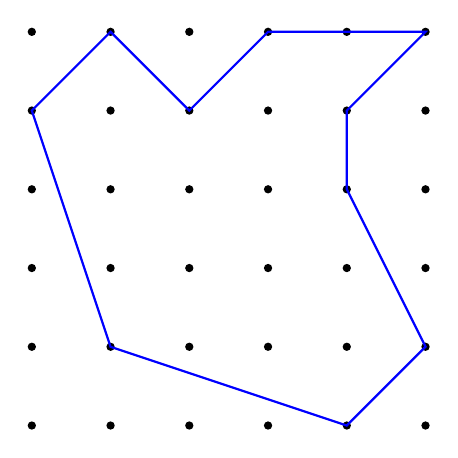
\begin{tikzpicture}

% testing:
%\draw[gray] (1,1) grid (6,6);

% grid of dots
\draw[mygrid] (1,1) grid (6,6);

% connect a path
\draw[thick,blue] (2,2) 
       -- (5,1)
       -- (6,2)
       -- (5,4)
       -- (5,5)
       -- (6,6)
       -- (5,6)
       -- (4,6)
       -- (3,5)
       -- (2,6)
       -- (1,5)
       -- cycle ;

\end{tikzpicture}
\end{document}
